\chapter{Architektura systemu}

Dobre zaprojektowanie architektury systemu jest fundamentalnym zadaniem. Na rynku istnieje wiele infrastruktur opartych na technologi przetwarzania w chmurze, które oferują bardzo podobne funkcjonalności. Należało wybrać te, które dawały najwięcej korzyści przy jak najniższej cenie (kosztorys omówiono w rozdziale 3). Dlatego zdecydowano się na Microsoft Azure. Dodatkowym atutem było to, że zespół miał już doświadczenie z tą usługą. Opis działania poszczególnych elementów systemu zostanie omówiony w dalszej części pracy.

\section{Schemat}

\begin{figure}[ht] %  figure placement: here, top, bottom, or page
   \centering
   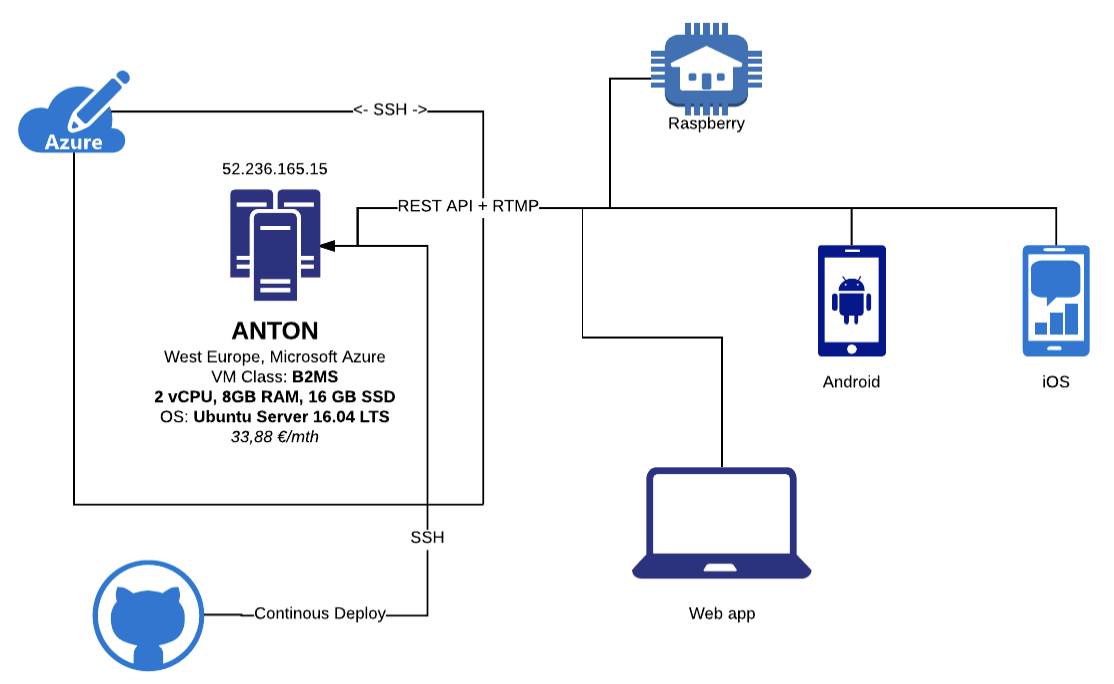
\includegraphics[width=12cm]{anton.png} 
   \caption{Schemat systemu [źródło własne]}
\end{figure}

Architektura została przedstawiona na schemacie (rys 2.1) . Wszystkie urządzenia klienckie(iOS, Android i Web) jak i Raspberry Pi komunikują się z serwerem ANTON wykupionym i pracującym na platformie Microsoft Azure. Komunikacja pomiędzy klientami a serwerem odbywa się dzięki REST API. Obraz natomiast przesyłany może być za pomocą dwóch protokołów RTMP i HLS. Postanowiono, że transmisja obrazu w systemie The Guard oparta będzie na protokole HLS ze względu na brak możliwości obsługi RTMP na iOS. Priorytetem było zapewnienie identycznych warunków i tych samych doświadczeń użytkownika na wszystkich platformach. Było to głównym powodem całkowitego odrzucenia przesyłania obrazu przy użyciu protokołu RTMP. RTMP posiada jednak w porównaniu do HLS jedną, aczkolwiek bardzo istotną przewagę. Jest to brak opóźnienia w transmisji obrazu. HLS wysyła dane w małych porcjach. Przed wysłaniem pierwszej części, konieczne jest jej nagranie. To właśnie powoduje kilkunastosekundowe opóźnienie w stosunku do RTMP, który transmituje obraz bezpośrednio. Oba protokoły omówiono dokładniej w rozdziale 4.3.

\section{Komunikacja}

Komunikacja pomiędzy elementami systemu odbywa się na zasadach architektury REST. Wiadomości przesyłane są asynchronicznie, na wskazane wcześniej adresy.
Takie podejście gwarantuje prostotę przesyłanych komunikatów oraz skalowalność w~kontekście nowych urządzeń Raspberry, strumieniujących dane, oraz nowych urządzeń korzystających z~aplikacji klienckich. Początkowo, projekt był oparty o~zapytania GET i~POST.  \cite{WEBARCH}

\paragraph{Zapytanie GET}
Metoda GET pozwala na pobranie dokumentu sieciowego, na postawie zapytania zawartego w~adresie URL. Metoda ta jest używana tylko i~wyłącznie do pobierania danych z~punktu docelowego. 

\paragraph{Zapytanie POST}
W metodzie POST, należy zamieścić wiadomość wewnątrz zapytania HTTP. Odpowiedzią na ten typ zapytania, może być zarówno kod statusu, jak i~dane, zwracane w podobnej postaci jak przy zapytaniu GET.

Wprowadzenie tokenów uwierzytelniających (więcej w akapicie nt. Bezpieczeństwa), spowodowało, że wymianę komunikatów oparto tylko i~wyłącznie na zapytaniach POST. Wysłanie takiego zapytania na określony adres powoduje uruchomienie specjalnej funkcji na serwerze. Każdy adres ma przypisaną osobną funkcję uruchamianą automatycznie po otrzymaniu zapytania. Funkcje te realizują operacje na bazie danych (CRUD) lub odpowiedzialne są za wysyłanie notyfikacji do wszystkich urządzeń klienta.
Obsługę zapytań można podzielić, ze względu na zaplanowane źródło zapytania: aplikacja użytkownika lub urządzenie Raspberry.
W~pierwszej kolejności przedstawione zostaną wiadomości wymieniane na linii Raspberry - Serwer.
\paragraph{a) Rejestracja Raspberry Pi:}
\begin{verbatim}
Adres: /backend/v1/devices/add
Zawartość:
{
	'serial': <serial-urządzenia>, 
	'name': <nazwa-urządzenia>, 
	'token': 'jwt.token.from.client'
}
\end{verbatim}
Działanie: Raspberry, o~podanym numerze seryjnym i~nazwie, zostaje dodane do bazy danych urządzeń.

\paragraph{b) Wykrycie ruchu:}
\begin{verbatim}
Adres: /backend/v1/PIRnotification
Zawartość: 
{
	'serial': <serial-urządzenia>, 
	'message': <wiadomość>, 
	'token': 'jwt.token.from.client'
}
\end{verbatim}
Działanie: Po odebraniu informacji o~wykryciu ruchu, następuje pobranie klatki ze strumienia obrazu nadawanego przez Raspberry o~wskazanym numerze seryjnym. Jeżeli na pobranej klatce wykryto człowieka, uruchamiana jest funkcja nagrywająca 30 sekundowy fragment wideo, który zostaje zapisany w~bazie danych Firebase Storage. Użytkownik zostaje poinformowany o~zajściu zdarzenia z informacją zawartą w polu 'message'. Notyfikacja zostanie wysłana jeżeli wykrycie ruchu zostało spowodowane przez człowieka. W każdym innym przypadku zostanie zignorowana.

\paragraph{c) Wykrycie zmian na czujniku:}
\begin{verbatim}
Adres: /backend/v1/notification
Zawartość: 
{
	'serial': <serial-urządzenia>, 
	'sensorType': <typ-czujnika>, 
	'value': <wartość>, 
	'token': `jwt.token.from.client`
}
\end{verbatim}
Działanie: Informuje serwer o wykryciu zagrożenia na jednym z~czujników. Serwer następnie wyszukuje wszystkich klientów, którzy posiadają urządzenie o numerze seryjnym, który wykrył niebezpieczne wskazania na czujniku i wysyła do nich powiadomienie za pomocą push notyfikacji. \newline
Następne zapytania dotyczą poleceń wysyłanych z~aplikacji użytkownika.
\paragraph{d) Pobranie urządzeń użytkownika:}
\begin{verbatim}
Adres: /backend/v1/get
Zawartość: 
{
	'owner':<użytkownik>, 
	'token': 'jwt.token.from.client'
}
\end{verbatim}
Działanie: Zwraca listę urządzeń użytkownika.
\paragraph{e) Zmiana nazwy urządzenia:}
\begin{verbatim}
Adres: /backend/v1/devices/changeRaspName
Zawartość:
{
	'serial': <serial-urządzenia>, 
	'name': <nowa-nazwa>, 
	'token': 'jwt.token.from.client'
}
\end{verbatim}
Działanie: Zmienia nazwę urządzenia, wyświetlaną w~aplikacji użytkownika. Przyjęto, że nazwa ta powinna oznaczać miejsce, w którym znajduje się urządzenie.
\paragraph{f) Uzbrojenie/rozbrojenie urządzenia:}
\begin{verbatim}
Adres: /backend/v1/devices/changeIsArmed

Zawartość: 
{
	'serial': <serial-urządzenia>, 
	'armed': <nowy-stan>, 
	'token': 'jwt.token.from.client'
}
\end{verbatim}
Działanie: Ustala czy nowe powiadomienia związane z~urządzeniem dalej będą wysyłane do aplikacji.
\paragraph{g) Pobranie listy notyfikacji:}
\begin{verbatim}
Adres: /backend/v1/devices/getNotifications
Zawartość: 
{
	'serial': <serial-urządzenia>,  
	'token': 'jwt.token.from.client'
}
\end{verbatim}
Działanie: Pobiera listę notyfikacji (historię zdarzeń) powiązanych z urządzeniem o podanym numerze seryjnym.
\paragraph{h) Powiązanie aplikacji z kontem użytkownika:}
\begin{verbatim}
Adres: /backend/v1/devices/fcmTokenUpdate
Zawartość: 
{
	'email': <użytkownik>, 
	'fcmToken': <token-z-firebase>, 
	'deviceId' : <id_aplikacji>
}
\end{verbatim}
Działanie: Powiązuje aplikację mobilną jak i~sesję aplikacji przeglądarkowej o~podanym tokenie z~kontem użytkownika. Dzięki temu, notyfikacje trafiają na wszystkie urządzenia użytkownika.
\newline
\newline
Wybrane rozwiązanie pozwala na łatwą lokalizację ewentualnego błędu w działaniu systemu oraz szybką jego naprawę. Ponadto prosta logika oraz łatwe i krótkie funkcje obsługujące zapytania sprawiają, że dalszy rozwój tej części systemu będzie możliwy bardzo niskim nakładem sił. 

\section{Bezpieczeństwo}

Aplikacje wysyłając zapytania do serwera muszą potwierdzić swoją tożsamość. 
W aplikacjach mobilnych zastosowano proponowane przez Firebase rozwiązanie JSON Web Tokens. W~momencie wysłania zapytania POST do serwera, aplikacja wysyła także unikalny token, który następnie jest przez serwer weryfikowany przy użyciu Firebase Admin SDK.

W~przypadku aplikacji internetowej, zastosowano wbudowane w bibliotekę Django zabezpieczenia: CSRF token oraz przesyłanie id sesji wraz z zapytaniem. Zabezpieczenie CSRF tokenem uniemożliwia tzw. `Cross Site Request Forgery' tj. ataki w~których na stronie, gdzie zalogowany jest użytkownik bez jego wiedzy uruchamiany jest skrypt, najczęściej w języku JavaScript. Następnie, korzystając z~faktu, że użytkownik jest zalogowany, wysyłane jest zapytanie na serwer, które może zrobić wszystkie operacje do których upoważniony jest dany użytkownik. CSRF token zapisywany jest w przeglądarce jako `ciasteczko' (eng. cookie) i jest dołączany do danych przesyłanych w momenie kliknięcia przycisku odpowiedzialnego za przesłanie formularza. Następnie wbudowana w serwer Django biblioteka weryfikuje na podstawie zapisanych i przesłanych danych sesji poprawność tokenu i w przypadku błędu zwraca błąd serwera 403.
Ponieważ token przy każdym zapytaniu jest tworzony na nowo na podstawie otwartej sesji, rozwiązanie nie było komfortowe dla użytkowników aplikacji mobilnych: aplikacja musiałaby najpierw ustanowić połączenie z serwerem (wysłać zapytanie GET na stronę główną), następnie zalogować się (wysłać zapytanie POST z danymi logowania) oraz zapisywać tokeny i id sesji odsyłane przez serwer. Aby ograniczyć ilość zapytań wysyłanych do serwera, posłużono się powyżej opisaną metodą tokenów JWT.
